
%%% This is a framework similarly to the mathematical one, but using the popular
%%% Cormen formatting for writing algorithms, much better than algorithm2e from latex if you ask me

\documentclass[12pt,a4paper]{article}

%This is useful specially for those who use Romanian characters
\usepackage[utf8x]{inputenc}
\usepackage{ucs}
\usepackage[romanian]{babel}

%All the math symbols stuff, you can comment those which you do not use!
\usepackage{amsmath}
\usepackage{amsthm}
\usepackage{amssymb}
\usepackage{amsfonts}
\usepackage{amssymb}

% Include support for graphics
\usepackage[pdftex]{color,graphicx}

% You will see some graphics magic with this, I am not drawing, just writing code!
\usepackage{tikz}

% For the code, it is mandatory to have the file clrscode3e.sty 
\usepackage{clrscode3e}

% Include support for linking table of contents to sections, footnotes & other hyperlinks
\usepackage[bookmarks]{hyperref}
% You can format the colors as you wish, here is an example:
% \hypersetup{unicode=true,%
% 	colorlinks=true,%
% 	citecolor=red,%
% 	filecolor=green,%
% 	linkcolor=black,%
% 	urlcolor=blue}

% Decomment this if you want to indent first paragraph
%\usepackage{indentfirst}

%To use headers, find out more about fancyhdr package :) 

%Info
\title{My cool report or essay for algorithms course}
\author{Name Surname}

% Ok, command names are suggestive, this is if you want to customize your documents 
% keywords or let LaTeX use it's default ones
% Decomment what are you interested in

% \renewcommand{\dateseparator}{.}
% \ddmmyyyydate
% \renewcommand{\contentsname}{Cuprins}
% \renewcommand{\figurename}{Figura}
% \renewcommand{\tablename}{Tabelul}

% Definition, theorem, proof, lemma & other crappy enivronments from the same category
% Decomment what are you interested in

% \newtheorem{definition}{Definiția}
% \numberwithin{definition}{section} % Definitia (SECTION_NO.DEFINITION_COUNT)
% 
% \newtheorem{theorem}{Teorema}
% \numberwithin{theorem}{section}
% 
% \newtheorem{lema}{Lema}
% \numberwithin{lema}{section}
% 
% \renewcommand{\proofname}{\underline{Demonstrație}}
% \renewcommand{\qedsymbol}{$\blacksquare$}

% Equation formatting for writing more beautiful and visible equations (in my opinion!! 
% There might be some other cooler options out there)
\everymath{\displaystyle} % All equations have displaystyle so no worry about forgetting this before a complicated equation
\numberwithin{equation}{section}  % Equation (SECTION_NO.EQ_COUNT)
%Syntax for this: \DeclareMathSizes{textsize}{mathsize}{subscriptsize}{subscriptscriptsize}
\DeclareMathSizes{13}{23}{13}{9}

\begin{document}
  \maketitle
 \newpage
 \tableofcontents
  \newpage
  
  \section{Sample CLRS cool algorithms}
  
  \begin{codebox}
 \Procname{$\proc{BubbleSort}(A)$}
  \li \For $i \gets 1$ \To $\attrib{A}{length} - 1$
  \Do
      \li \For $j \gets \attrib{A}{length}$ \Downto $i + 1$
      \Do
	  \li \If $A[j] < A[j - 1]$ 
	   \Do
	   \li   exchange $A[j]$ with $A[j - 1]$
	    \End
	\End
   \End
\end{codebox}

\begin{codebox}
 \Procname{$\proc{cmMdc}(x,y)$}
  \li $b \gets y; \; a \gets x; \; r \gets y; $
  \li \While ($b \neq 0$)
      \Do
	  \li $r \gets a \mod b$
	   \li $a \gets b$
	   \li $b \gets r$
      \End
  \li \Return $x$
\end{codebox}

\begin{codebox}
 \Procname{$\proc{Vertex-Cover}(k, G = (V, E))$}
  \li $i \gets 0$ \li $S \gets \emptyset$
  \li \While($i \le k$) \Do
  \li $i \gets i + 1$
  \li $v \gets \proc{choice}(V)$
  \li $S = S \cup \{v\}$
  \End
  \li 
\If ($\proc{isVertexCover(S, E)} \isequal \const{true}$)
\li
\Then
\Return succes
\li
\Else
\Return fail
\End
\end{codebox}
  
 \section{Sample Recurrence tree}
 
I want recurrence tree for equation $T(n) = T \left( \frac{n}{2} \right) + T \left(   \frac{n}{4} \right) + \Theta(n^2)$. \\

Say $f(n) \in \Theta (n^2), f(n) = cn^2, c \in \mathbb{R}_+$. Recurrence equation is: $T(n) = T \left(   \frac{n}{2} \right) + T \left(   \frac{n}{4} \right) + cn^2$

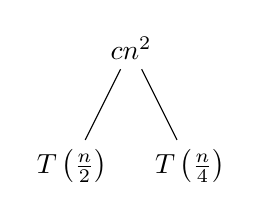
\begin{tikzpicture}
  \node {$cn^2$}
    child {node {$T \left(   \frac{n}{2} \right)$}
    }
    child {node {$T \left(   \frac{n}{4} \right)$}
    };

\end{tikzpicture} $\ \ \  \ \   \ \  \ \  \ $
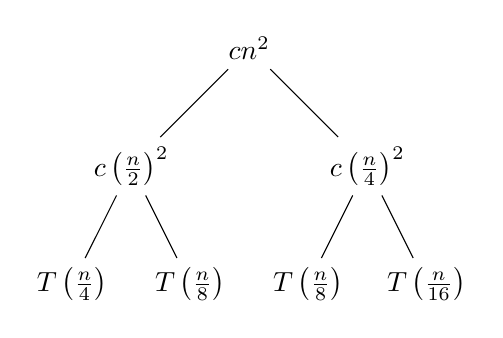
\begin{tikzpicture}[level distance=1.5cm,
  level 1/.style={sibling distance=3cm},
  level 2/.style={sibling distance=1.5cm}]

  \node {$cn^2$}
    child {node {$c\left(   \frac{n}{2} \right)^2$}
      child {node {$T \left(   \frac{n}{4} \right)$}}
      child {node {$T \left(   \frac{n}{8} \right)$}}
    }
    child {node {$c\left(   \frac{n}{4} \right)^2$}
    child {node {$T \left(   \frac{n}{8} \right)$}}
      child {node {$T \left(   \frac{n}{16} \right)$}}
    };
\end{tikzpicture} \\

Recursion tree (I know it's not perfect!):

\begin{center}
\begin{tikzpicture}[level/.style={sibling distance=72mm/#1},node distance=5cm, level distance = 1.5cm, level 3/.style={sibling distance=1.5cm}, level 4/.style={sibling distance=1cm}]

\node {$cn^2$} 
child {node {$c \left(   \frac{n}{2} \right)^2$} 
child {node {$c \left(   \frac{n}{4} \right)^2$} 
child {node {$c \left(   \frac{n}{8} \right)^2$}
    child {node {$\ldots$}
	child {node {$T(1)$}}
    }
    child {node {$\ldots$}}
} 
child {node {$c \left(   \frac{n}{16} \right)^2$}
    child {node {$\ldots$}}
child {node {$\ldots$}}} 
} 
child {node {$c \left(   \frac{n}{8} \right)^2$} 
child {node {$c \left(   \frac{n}{8} \right)^2$}
child {node {$\ldots$}} 
child {node {$\ldots$}} } 
child {node {$c \left(   \frac{n}{16} \right) ^ 2$}
    child {node {$\ldots$}}
child {node {$\ldots$}}
} 
} 
} 
child {node {$c \left(   \frac{n}{4} \right)^2$} 
child {node {$c \left(   \frac{n}{8} \right)^2$} 
child {node {$\vdots$} } 
child[fill=none] {edge from parent[draw=none]} 
} 
child {node {{$c \left(\frac{n}{16} \right)^2$}}
  child {node {$\ldots$}
    child {node {$\ldots$}}
child {node {$\ldots$}} 
}
child {node {$\ldots$} 
child {node {$\ldots$}}
child {node {$T(1)$}}}
} 
}; 
\end{tikzpicture}
\end{center}

\section{Sample flowchart of a stack implemented as an array}

\begin{figure}[hb]
 \begin{center}
  \begin{tikzpicture}[node distance=2.5cm, start chain=going below,]
   % nodes
   \node[block] (a)                                     {\begin{tabular}{|c|}\hline 1 \\\hline \end{tabular}};
   \node[block] (b)  [right of=a, node distance=4.3cm] {\begin{tabular}{|c|c|}\hline 1 & 2 \\\hline \end{tabular}};
   \node[block] (c)  [right of=b, node distance=4.3cm]  {\begin{tabular}{|c|c|c|}\hline 1 & 2 & 3 \\\hline \end{tabular}};
   \node[block] (d)  [right of=c, node distance=4.3cm]  {\begin{tabular}{|c|c|c|c|}\hline 1 & 2 & 3 & 4\\\hline \end{tabular}};
  
   % edges
   \draw[->] (a) -- node[above] {insert} node[below] {copy} (b);
   \draw[->] (b) --node[above] {insert} node[below] {copy}  (c);
   \draw[->] (c) -- node[above] {insert} node[below] {copy} (d);
 
  \end{tikzpicture}

  \label{flowchart}
 \end{center}
\end{figure}
  
\end{document}

